\chapter{Implementation}
\label{chp:Implementation}

\section{Embedded Software of Camera}
One of the main reasons behind choosing the OV2640 CMOS sensor is that it has a ready electronic interface that can be used t interface with standard 8-bit/16-bit microcontrollers,  The OV2640 is one of the sensors that is available as a part of Arducam hardware. Arducam is an open source camera that comes along with open-source hardware and software that is needed to capture images using the CMOS sensor. However, using the camera comes with its own advantages and disadvantages. The main advantage behind using this platform is that the platform has open-source libraries that could be used to interface with ATMEGA328P, an 8-bit microcontroller. In space-missions, it would not be possible to send high-powered microprocessors, and microcontroller is used as an on-board computer. Arducam has standard software libraries that can be used to interface with Arduino making the cumbersome and lengthy job of writing an interface software to a CMOS sensor way more easier.  A disadvantage of the hardware module is the on-board memory that it has to capture an image. The OV2640 Arducam mini camera module can capture upto 1600*1200 resolution images with or without any form of compression. However due to the limitation of the on-board OV2640 FIFO memory AL422B it would be possible to capture only compressed images and not full resolution RAW images. The AL422B on-board FIFO has only 384KB of memory and that is not enough to obtain a full-resolution RAW image. However, we would like to have the RAW unprocessed image from the sensor. One of the other disadvantages is that custom code needs to be written to obtain various controls that we need for our camera. We have to write our own camera control software if we need to control factors such as exposure time, ISO, etc. as the default software uses automatic exposure control to enhance the image quality. The camera module architecture is shown in Figure \ref{fig:arducam_arch}.

 \begin{figure}[!htbp]
\centering
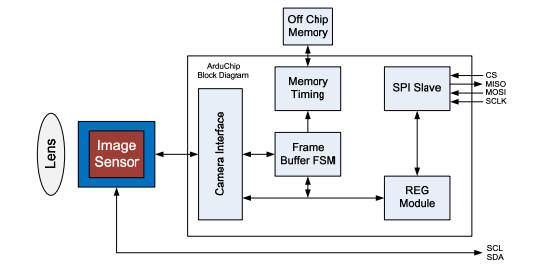
\includegraphics[scale=0.75]{pics/arducam_architecture}
\caption{Camera Architecture of Arducam Mini OV2640 Camera Module}
\label{fig:arducam_arch}
\end{figure}

The system for experiments is as shown in Figure \ref{fig:imp_setup}. The Arduino is connected to the camera module through an I2C interface. Using the I2c interface it possible to set registers that control the functioning of the camera such as the output format, digital signal processing, etc. SPI interface is used to transfer the image data from the camera module to the Arduino. The Arduino upon receiving the image data either writes it to an  SD card or sends it to the software on the PC through the USB connection. 
\begin{figure}[!htbp]
\centering
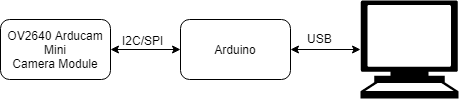
\includegraphics[scale=0.75]{pics/implementation_setup}
\caption{Implementation Setup}
\label{fig:imp_setup}
\end{figure}


\subsection{Exposure Control of OV2640}
In order to do experiments, it was required to control the exposure of the camera. In the default driver that was provided by the vendor, the exposure was automatically set using the Automatic Exposure Control (AEC) feature in the sensor. So, a modification was needed in the driver software. Fortunately, the driver is open source and the there were libraries that could assist in setting the on-board registers through the I2C interface on the Arduino. First, let us have a look at how exposure control works in an OV2640 camera. All rolling shutter image sensors including OV2640 exposure the sensor one-line at a time i.e. pixels in the same line are exposed at the same time and different pixels in different lines are exposed at a different time. So, the minimum exposure time would be one line time and the maximum exposure time would be the frame time. This is illustrated in Figure \ref{fig:RollingShutterOV2640}. By default the pixel clock is set at 36MHz. We can calculate the minimum line time using the following equation:

$$
Minimum Exposure Time = 1/Pixel Clock * Pixel Clockes per line 
$$
As shown in Figure \ref{fig:ShutterTimingOV2640}, one line consists of 1922 pixel clocks(1600 for pixel data and 322 clocks of horizontal blanking). So the minimum exposure time would be 53.39$\mu$seconds and the maximum exposure time would be the frame time(multiply line time by 1200 + 44 lines of vertical blanking) which would be 66.63ms\cite{RollingShutterOV2640}. In order to control the exposure of the camera it is necessary to modify registers of address 4, 10, 13, 45. So, these registers were modified according the the required exposure time value. The driver software on the Arduino was modified to obtain different exposure times.
\begin{figure}[ht]
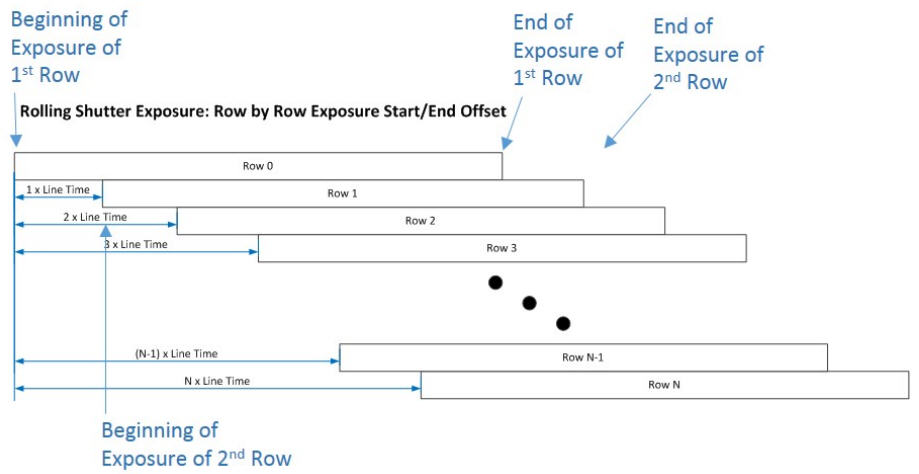
\includegraphics[width=\textwidth]{pics/rolling_shutter}
\caption{Rolling Shutter Operation on OV2640\cite{RollingShutterOV2640}}
\label{fig:RollingShutterOV2640}
\end{figure}

\begin{figure}[ht]
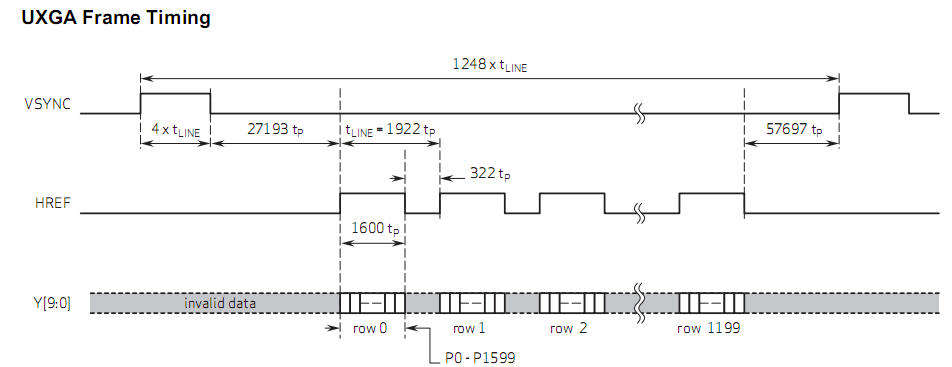
\includegraphics[width=\textwidth]{pics/OV2640timing}
\caption{Shutter Timing Diagram of OV2640\cite{RollingShutterOV2640}}
\label{fig:ShutterTimingOV2640}
\end{figure}

    \begin{figure}[ht]
    \centering
    \begin{subfigure}{0.5\textwidth}
    \centering
        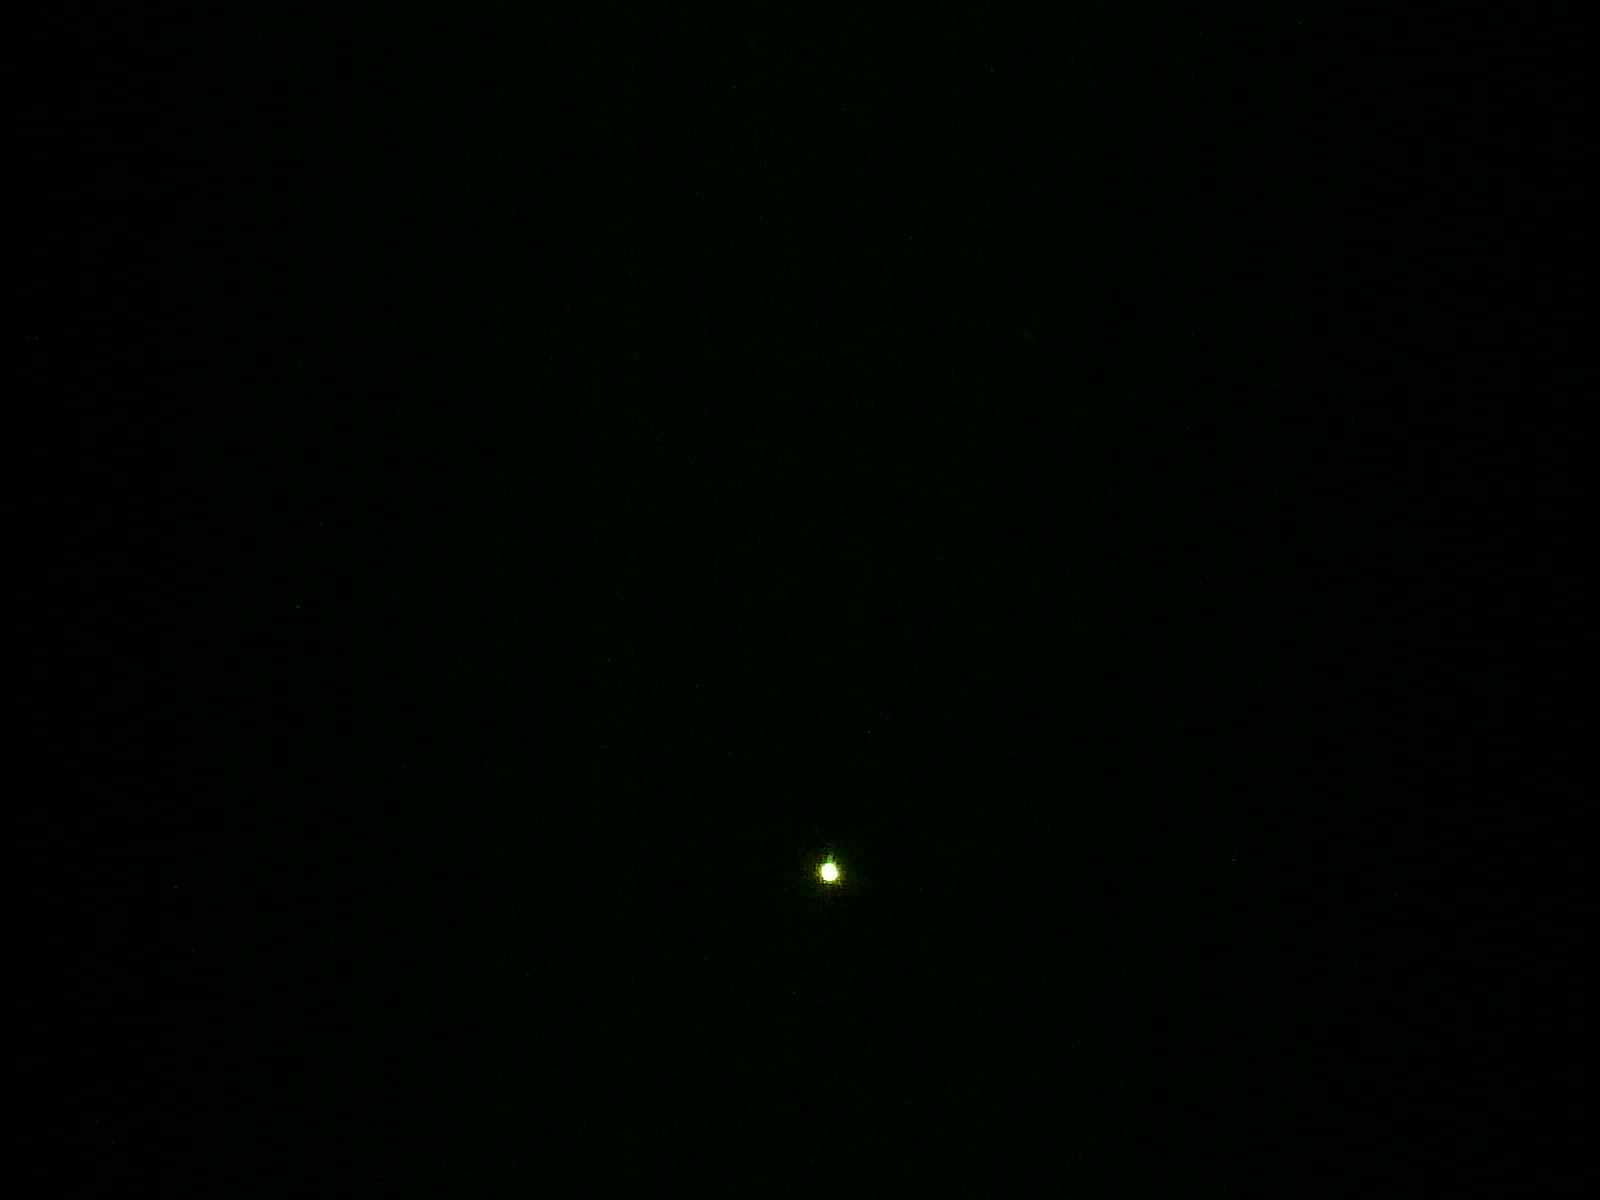
\includegraphics[width=0.5\linewidth]{pics/exposure/60us}
        \caption{60 $\mu$seconds}
        \label{fig:exp60us}
    \end{subfigure}%
    \begin{subfigure}{0.5\textwidth}
    \centering
        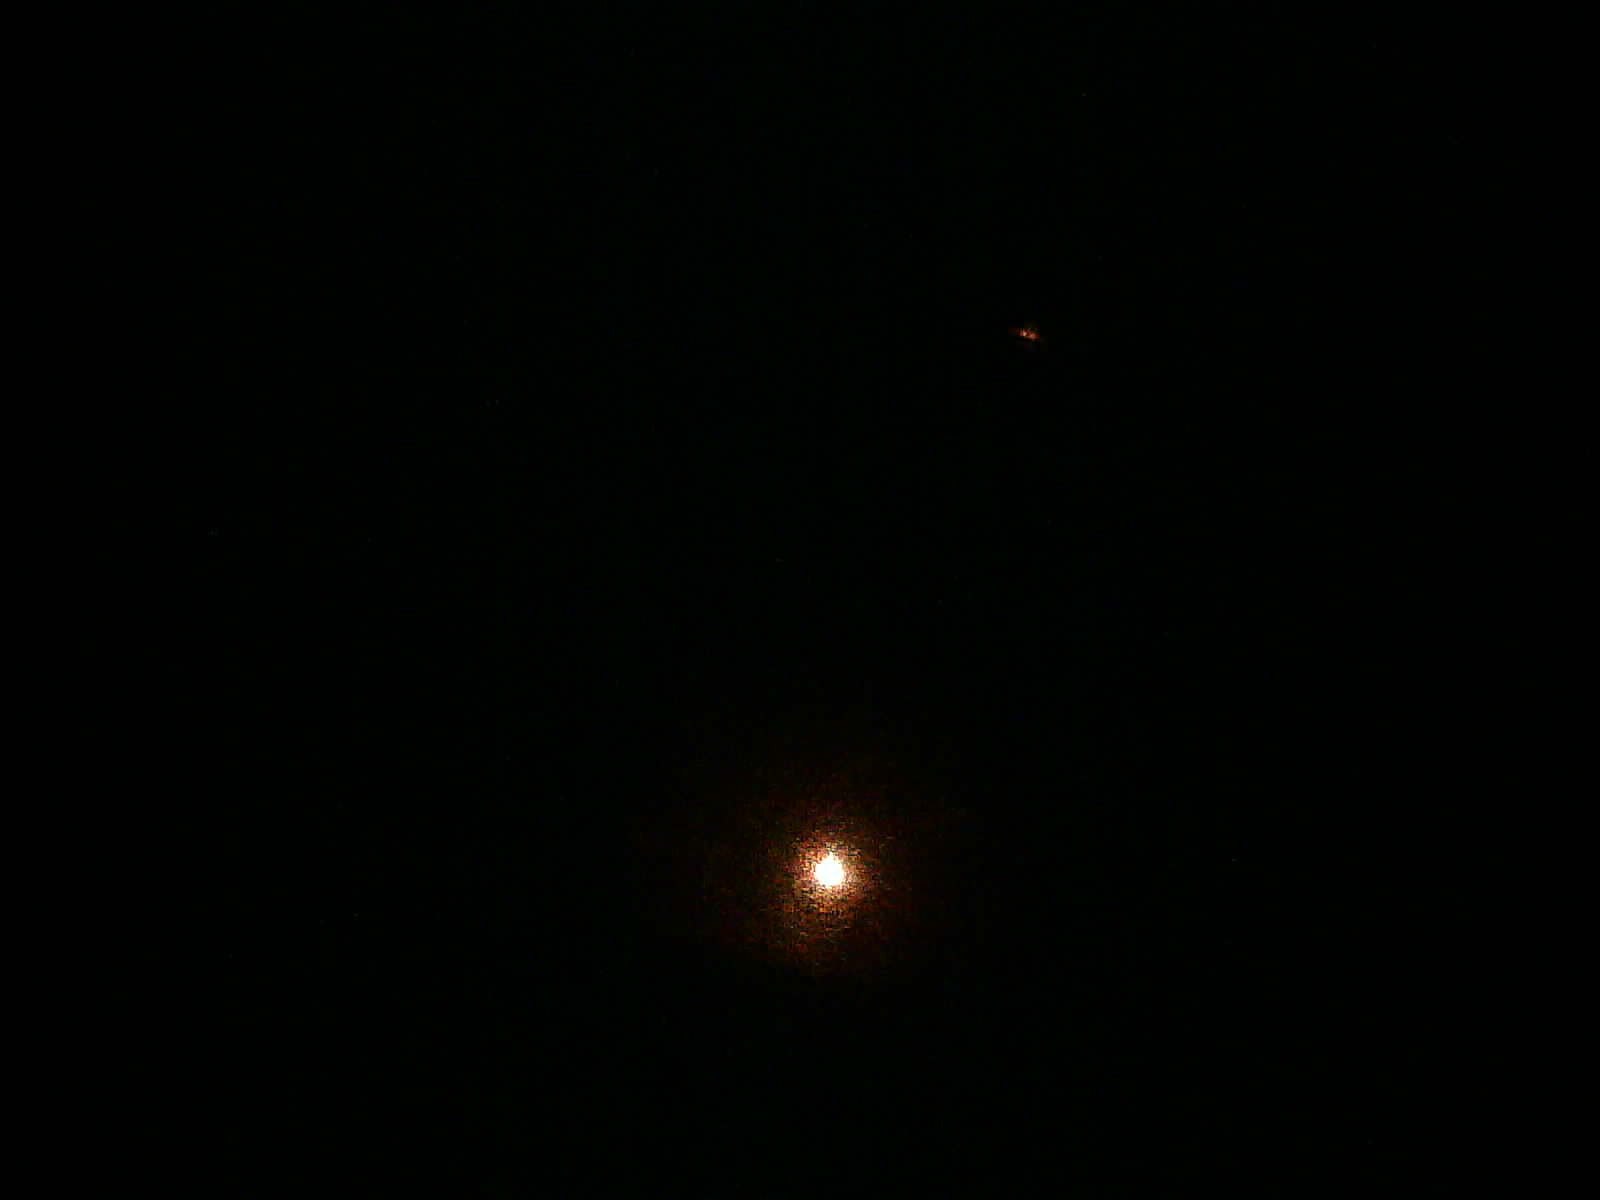
\includegraphics[width=0.5\linewidth]{pics/exposure/1ms}
        \caption{1ms}
        \label{fig:exp1ms}
    \end{subfigure}
    
    \begin{subfigure}{0.5\textwidth}
    \centering
        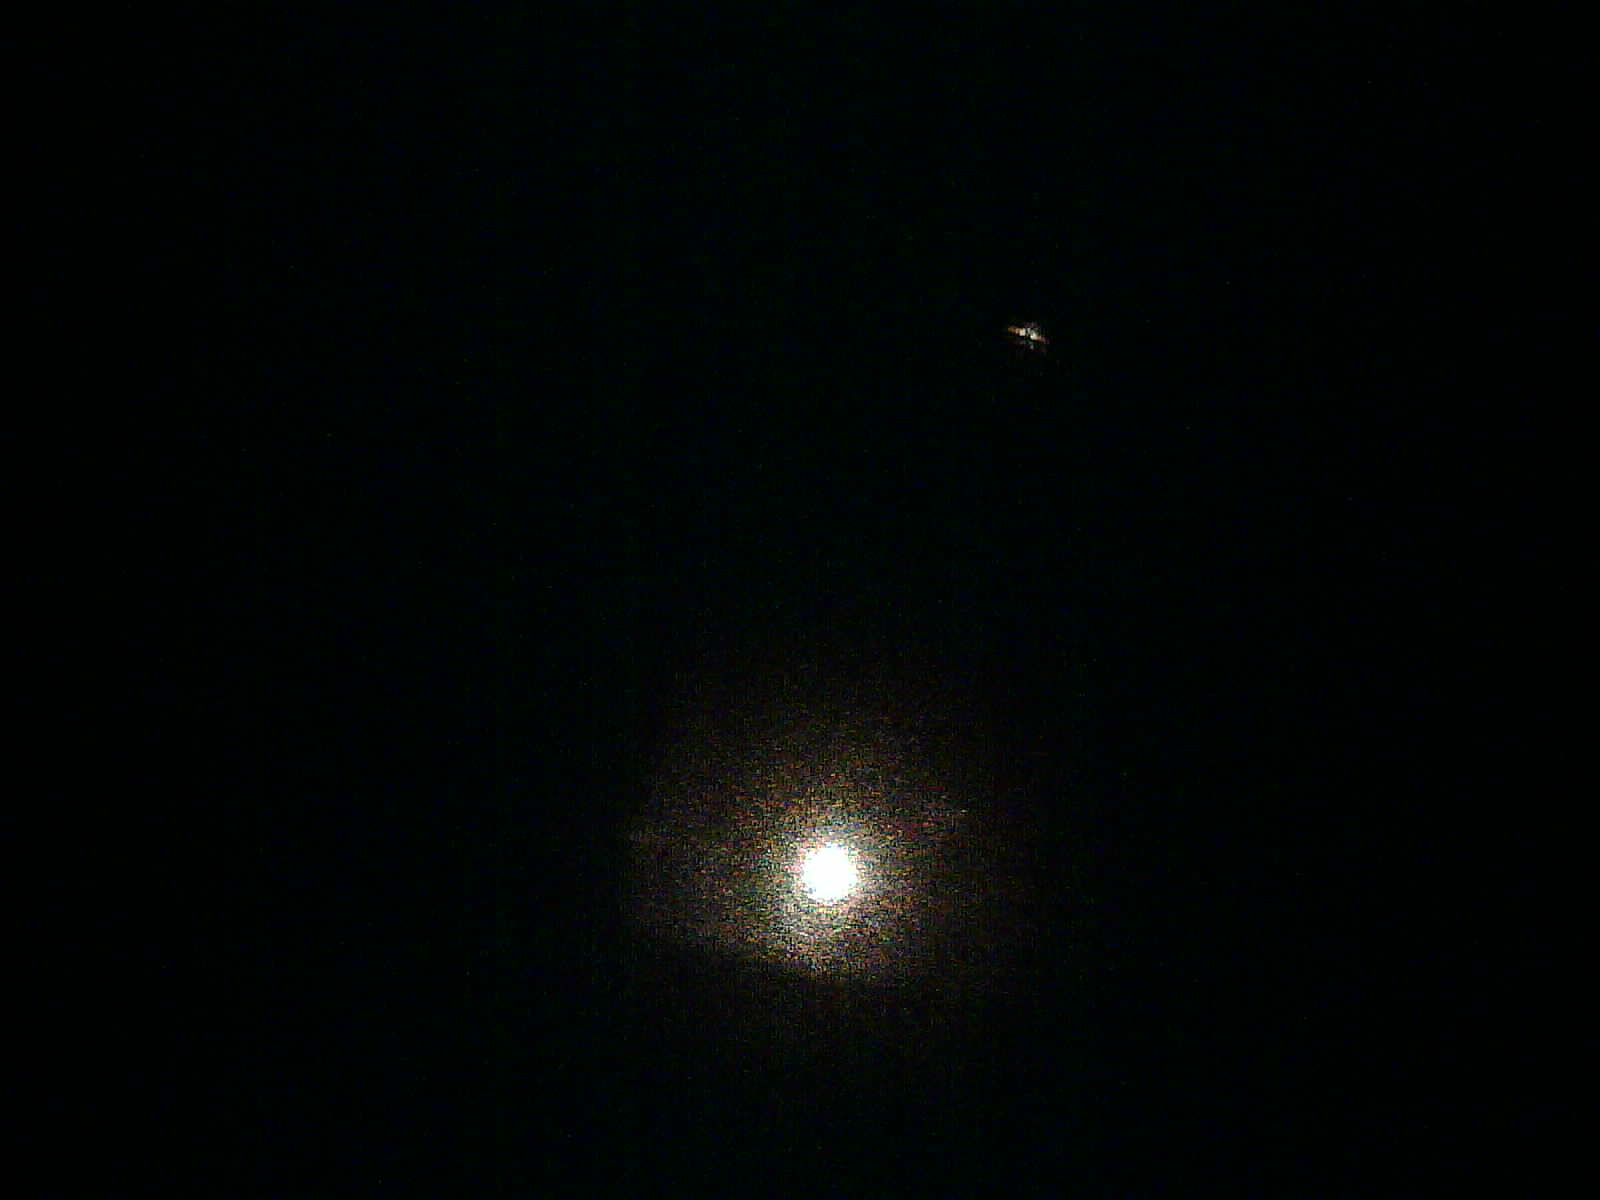
\includegraphics[width=0.5\linewidth]{pics/exposure/5ms}
        \caption{5ms}
        \label{fig:exp5ms}
    \end{subfigure}%
    \begin{subfigure}{0.5\textwidth}
    \centering
        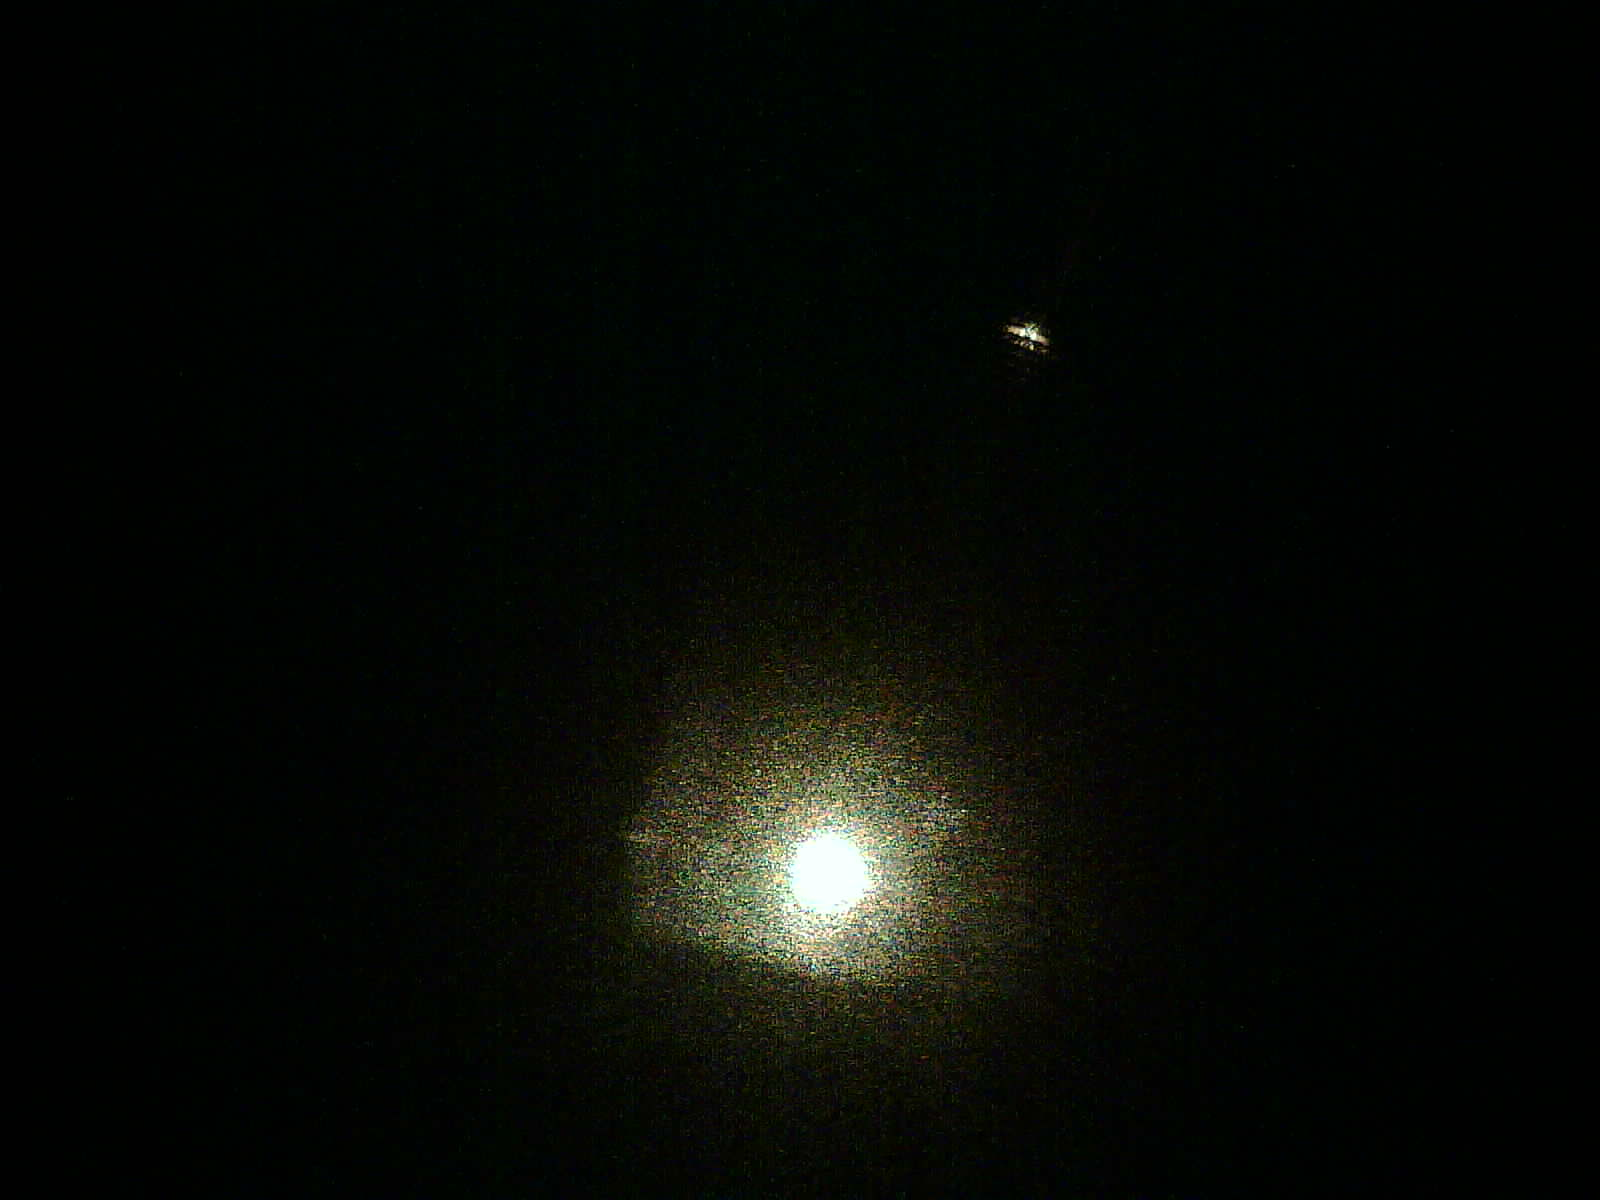
\includegraphics[width=0.5\linewidth]{pics/exposure/10ms}
        \caption{10ms}
        \label{fig:exp10ms}
    \end{subfigure}
        
        \begin{subfigure}{0.5\textwidth}
    \centering
        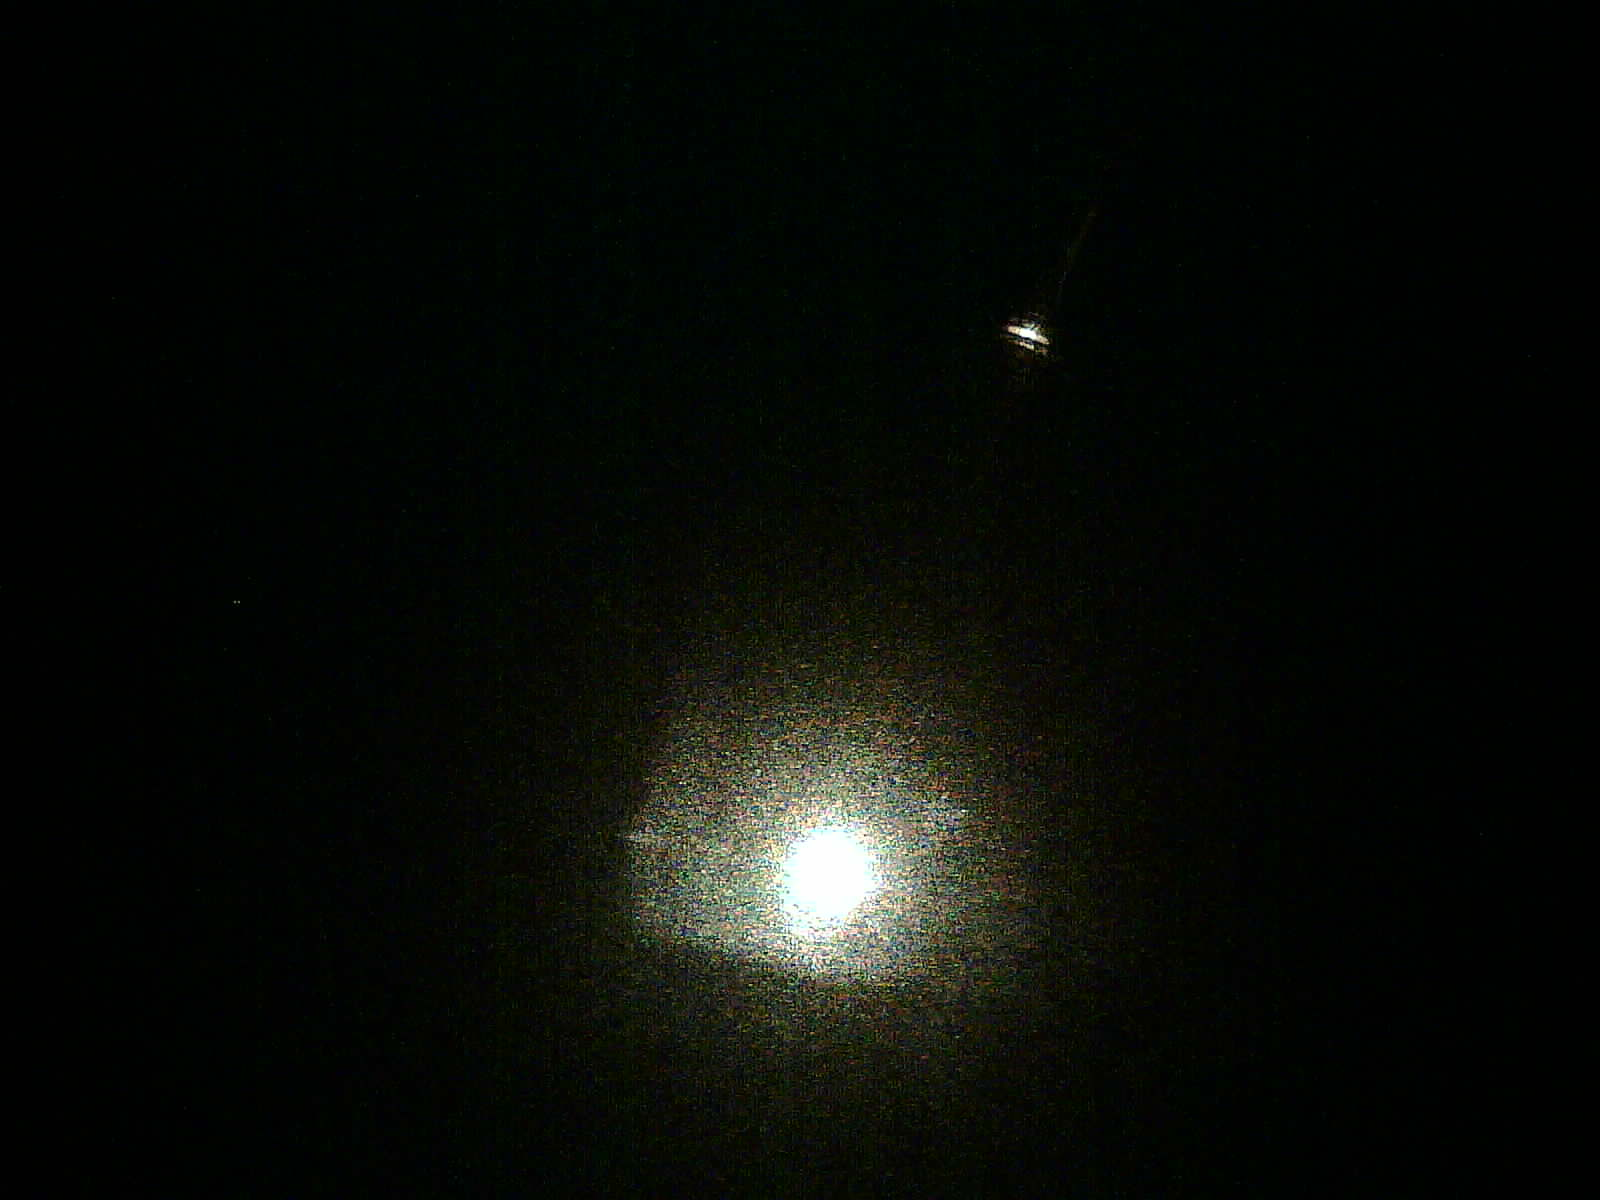
\includegraphics[width=0.5\linewidth]{pics/exposure/20ms}
        \caption{20ms}
        \label{fig:exp20ms}
    \end{subfigure}%
    \begin{subfigure}{0.5\textwidth}
    \centering
        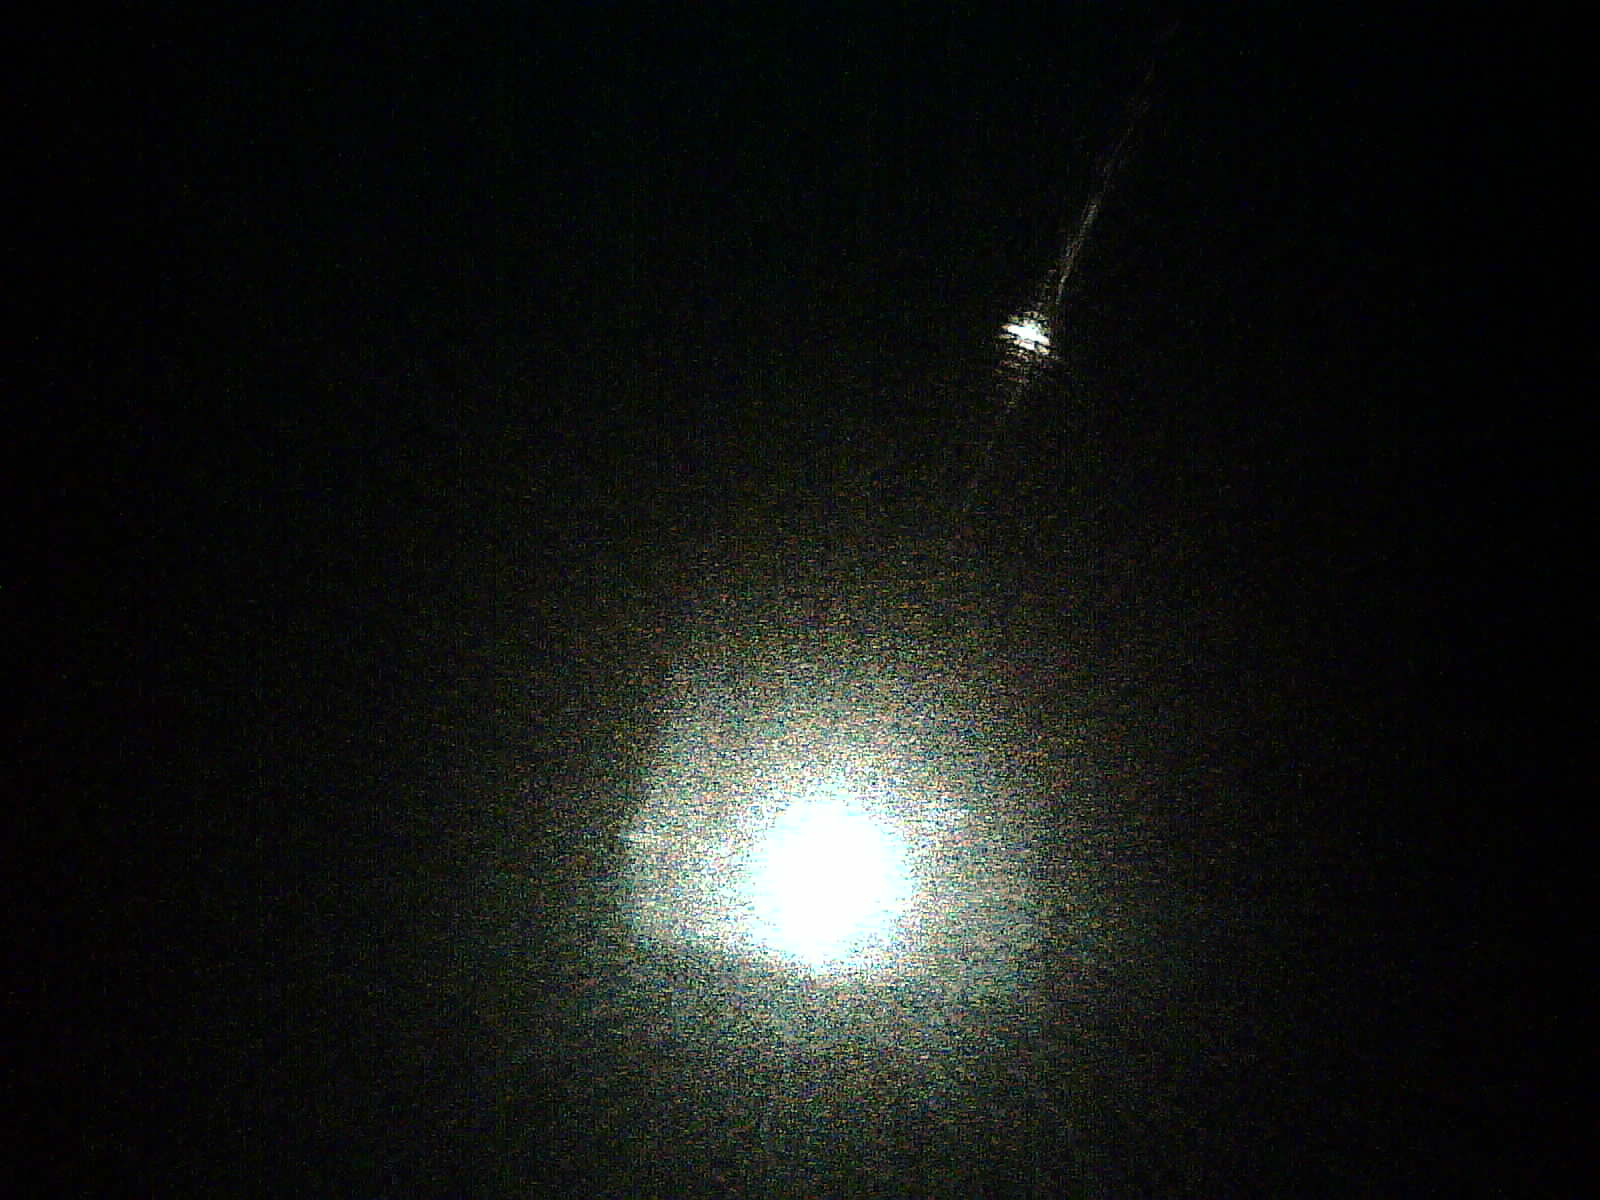
\includegraphics[width=0.5\linewidth]{pics/exposure/60ms}
        \caption{60ms}
        \label{fig:exp60ms}
        
    \end{subfigure}    
    \caption{Images of a laser beam caught in different exposure times(with lens)}
    \label{fig:exptests}
    \end{figure}

\section{Testing of Acceptance Cone of Sensor}
\subsection{Experimental Setup}
A study conducted previously\cite{cra2} has employed cat's eye reflectometer method using four spherical lenses to accurately measure the chief ray angle of a CMOS sensor upto 0.65 degrees\cite{cra2}. Apart from this, Armstring Optical another method for measuring the chief ray angle or the acceptance angle\cite{cra1} is proposed. However, our work employs a simpler method to measure the acceptance cone of a CMOS sensor without use of any lenses. Our method uses a collimated laser beam(650 nm), a pinhole for finding the accurate center of axis and a rotational stage(to measure angular rotation) to find the response of the sensor to light at different angles and in-turn the acceptance cone of the sensor. 
Figure \ref{fig:exp_acc} shows the experimental setup that was made to measure the acceptance cone of the sensor. A collimated laser beam was reflected off a mirror and it is passed through a pinhole. The pinhole was used because a diverged wave did not provide much information about the distribution of energy of the signal. Hence, a pinhole was introduced to focus the beam onto a reduced area on the sensor. The difference in measurements with and without pinhole is shown in Figure \ref{fig:pinholeDiff}.
 \begin{figure}[ht]
\centering
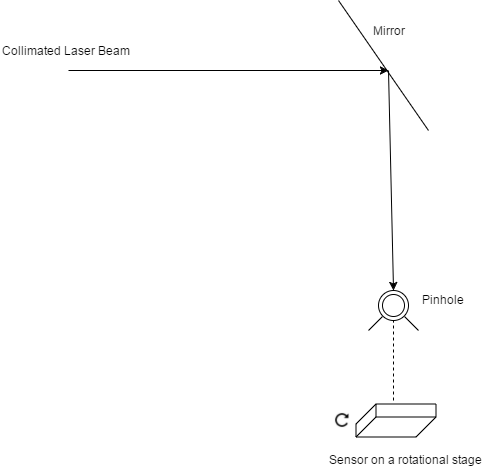
\includegraphics[scale=0.50]{pics/acceptanceCone.png}
\caption{Experimental Setup for detection of acceptance cone}
\label{fig:exp_acc}
\end{figure}

\begin{figure}[ht]
    \centering
    \begin{subfigure}{0.5\textwidth}
    \centering
        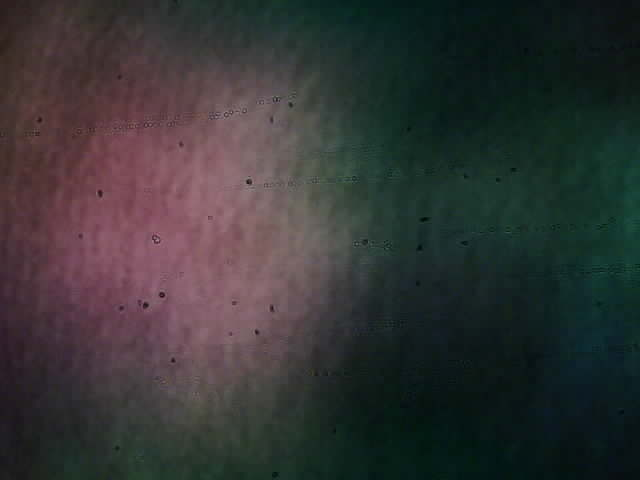
\includegraphics[width=0.5\linewidth]{pics/withoutPinhole.jpg}
        \caption{Image without pinhole}
        \label{fig:nopinhole}
    \end{subfigure}%
    \begin{subfigure}{0.5\textwidth}
    \centering
        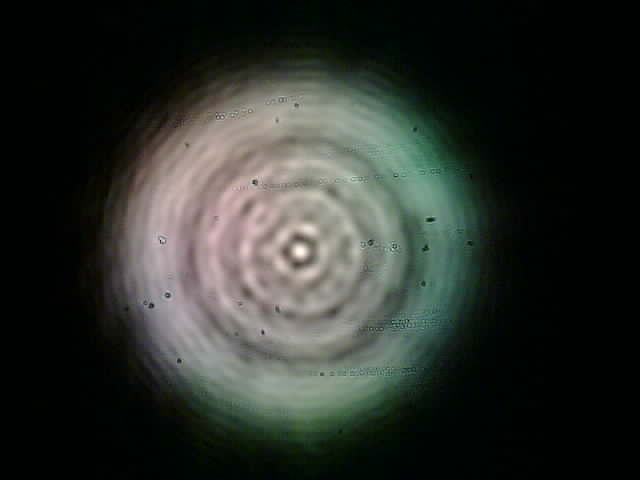
\includegraphics[width=0.5\linewidth]{pics/withPinhole.jpg}
        \caption{Image with pinhole}
        \label{fig:pinhole}
    \end{subfigure}
    \caption{Images of a laser beam caught with and without pinhole}
    \label{fig:pinholeDiff}
    \end{figure}
The pinhole cannot be used to measure the acceptance cone of the sensor because the waveform from the pinhole is a combination of different plane waves of different frequencies. Hence, the measurement was done without a pinhole. In order to measure the acceptance cone of the sensor, it is necessary to identify a portion of the image that can be taken as a reference to plot the variation in the signal measurement. It was assumed that the maximum point in the image can be taken as the signal. Since there was too much variation in the intensities measured, it was decided that we would average the 10 images in each angular position to reduce the signal noise. The maximum value in the image was taken and normalized and the measurements were repeated from -45 to +45 for 10 sets. The same image readings were used for finding out the response of different color channels(RGB). This experiment took a period of two weeks to complete. The exposure value was chosen such that the output does not saturate(does not reach 255) for any value in the image(See Figure \ref{fig:exp_acc_exp}). The maximum value in the image versus the angle is plotted. The ideal exposure value would be the one in which the the signal does not saturate and there is still some room for additional signals. This is also indicated in Figure \ref{fig:exp_acc_exp}.
\begin{figure}[ht]
\centering
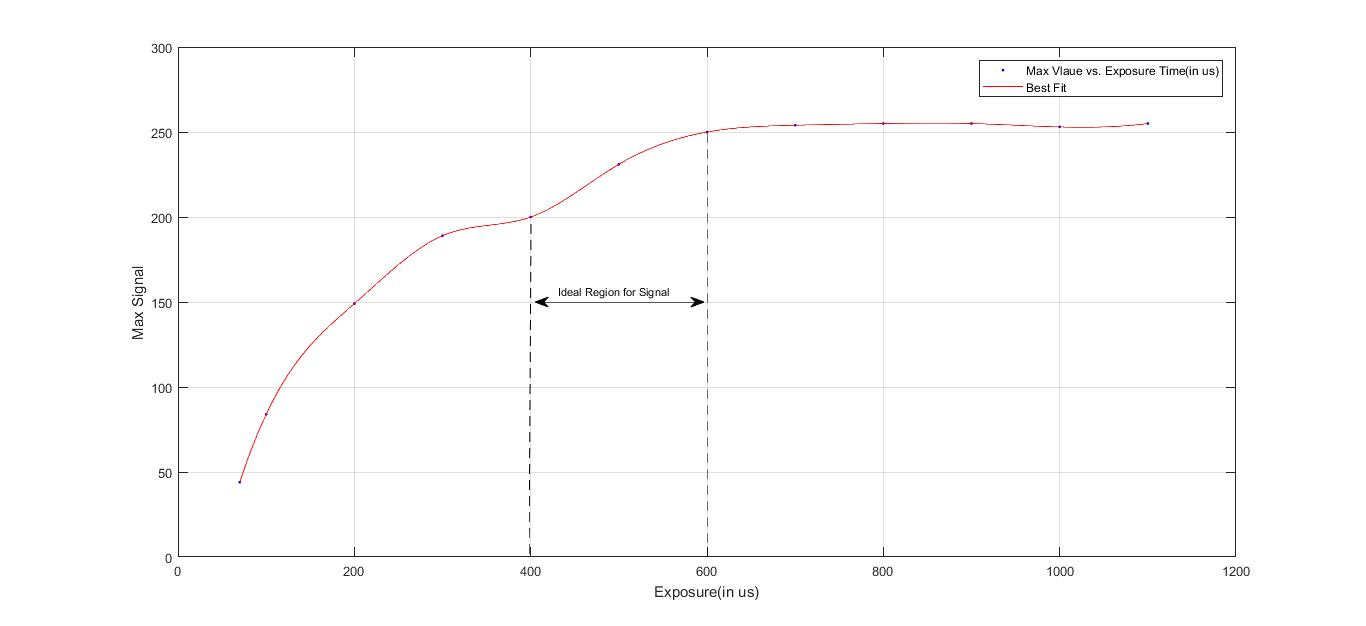
\includegraphics[scale=0.25]{pics/ExposureTests.jpg}
\caption{Response for different Exposure values in microseconds}
\label{fig:exp_acc_exp}
\end{figure}

The obtained response curves for each channel are shown in Figure \ref{fig:exp_acc_red_1}, \ref{fig:exp_acc_green_1}, \ref{fig:exp_acc_blu_1}. The normalized signal values are plotted with the standard deviation obtained for each angle are indicated with the use of an error bar. The best obtained curve fit is also plotted.
 \begin{figure}[ht]
\centering
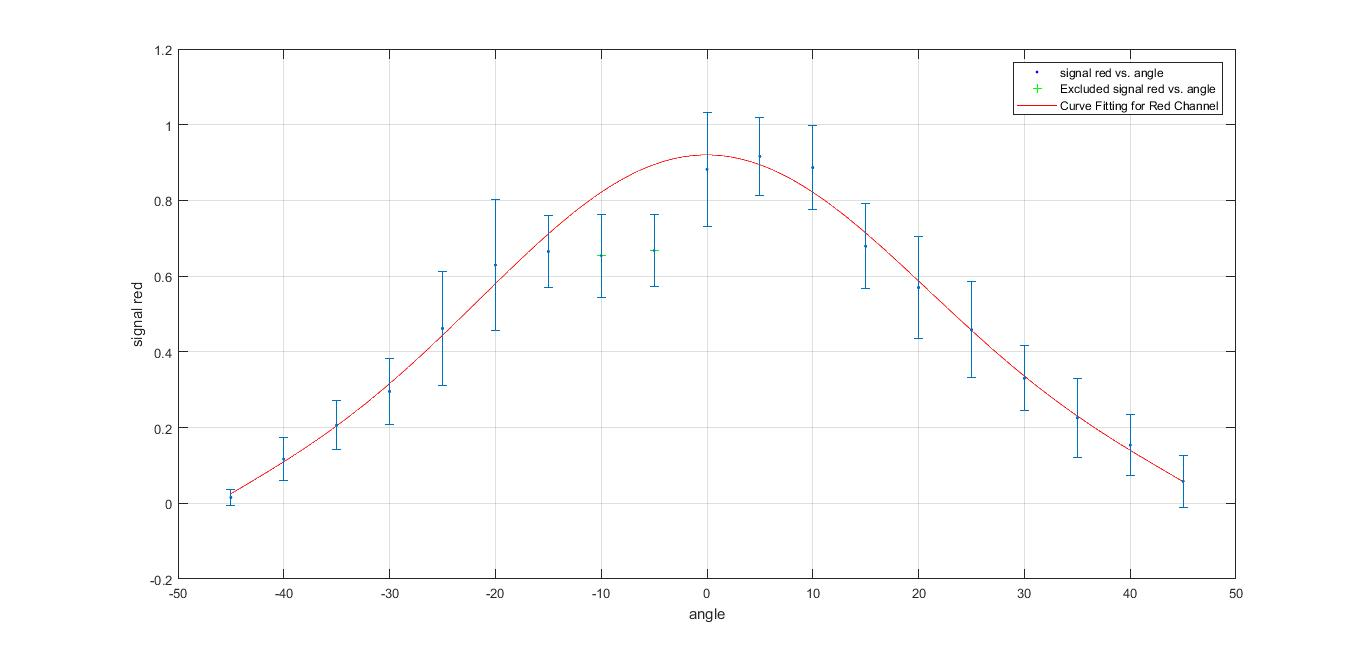
\includegraphics[scale=0.25]{pics/RedChannel.jpg}
\caption{Response for Red Channel in Initial Experiment}
\label{fig:exp_acc_red_1}
\end{figure}

 \begin{figure}[ht]
\centering
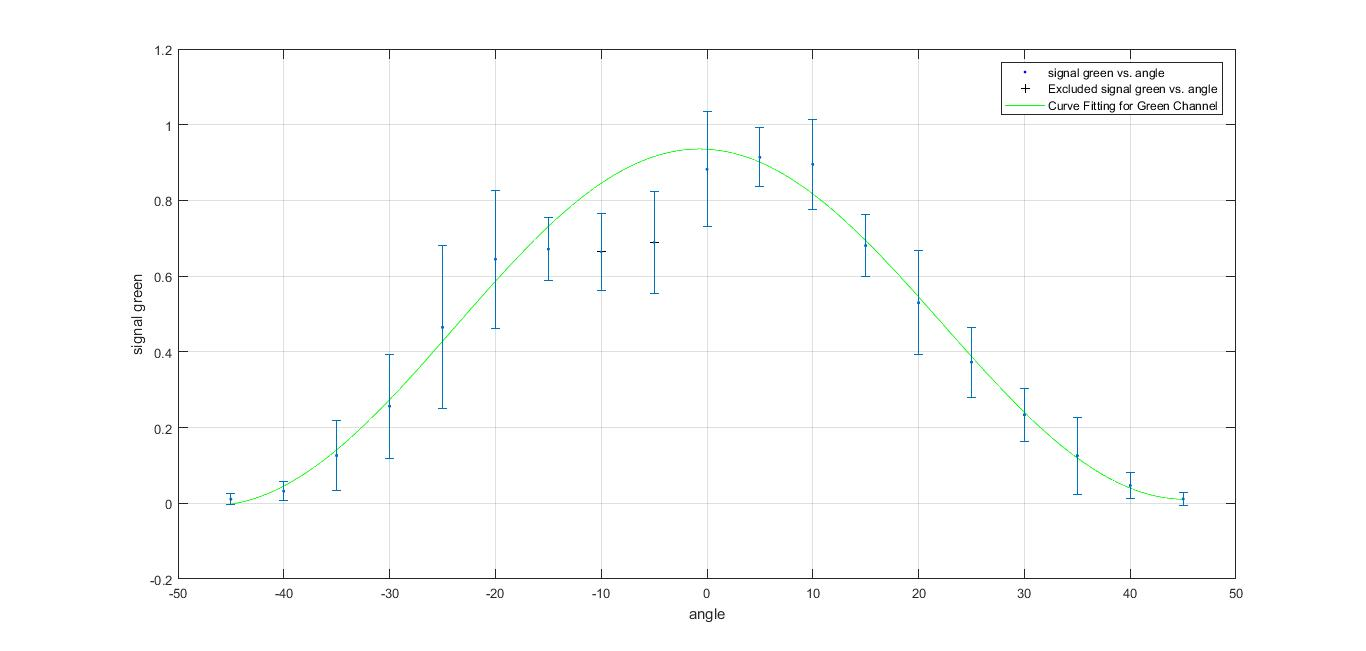
\includegraphics[scale=0.25]{pics/GreenChannel.jpg}
\caption{Response for Green Channel in Initial Experiment}
\label{fig:exp_acc_green_1}
\end{figure}

\begin{figure}[ht]
\centering
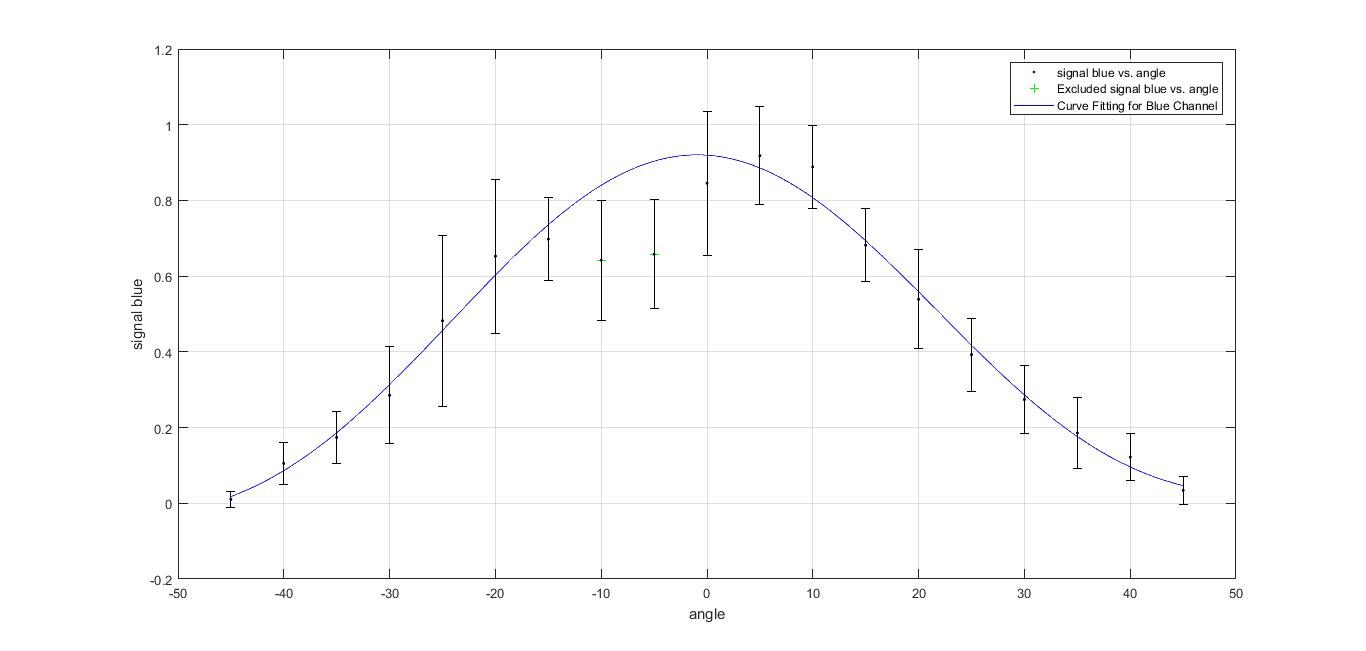
\includegraphics[scale=0.25]{pics/BlueChannel.jpg}
\caption{Response for Blue Channel in Initial Experiment}
\label{fig:exp_acc_blu_1}
\end{figure}
The initial observations from the results obtained are:
\begin{itemize}
\item There seems to be a very large standard deviation for each angle.
\item There seems to very sharp outliers at -5 and -10 degrees which is an highly unexpected behaviour.
\end{itemize}
These two observations point to experimental error. The error in the experimental results could be due to the following reasons:
\begin{itemize}
\item \textbf{Error introduced due to translation of the rotational stage :} In order to make sure that the beam always hits the stage is translated if the beam does not hit due to translation of the sensor away from the beam. This introduces an additional angular error which is not taken into account in the initial experiment. So, the stage was calibrated using the pinhole. If the sensor is exactly at the center of rotation of the rotational stage, the laser beam must always hit the same position of the sensor no matter what the rotational angle may be. The position of the sensor on the rotational stage was calibrated such that the signal(image with pinhole) obtained always remained at the center of the sensor. 

\item \textbf{Improper Reference Signal from Image :} At times, it was observed that the maximum point in the image occurs at different and unexpected points that are outside the beam. This also leads to different parts of the signal being measured each time. The outliers in the results could also mean that. An example average image in which the maximum is obtained at the end of the beam is shown in Figure \ref{fig:exp_acc_improper}. The point from where the signal is obtained is marked using a yellow star in the Figure \ref{fig:exp_acc_improper}.
\begin{figure}[ht]
\centering
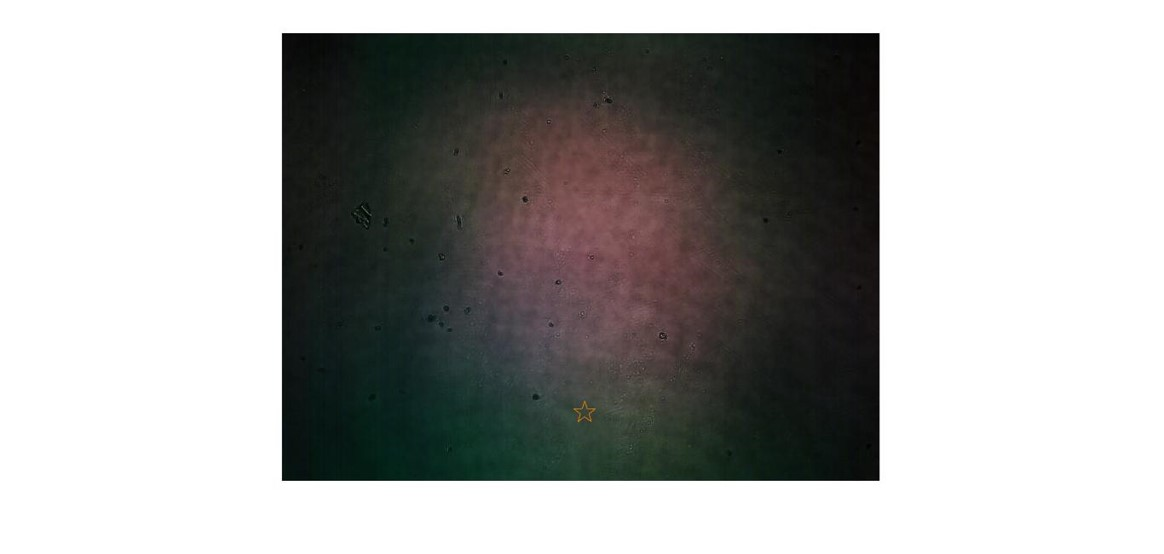
\includegraphics[scale=0.50]{pics/ImproperDetection.jpg}
\caption{Improper Reference Point for Signal}
\label{fig:exp_acc_improper}
\end{figure}
\item \textbf{Large Variation on intensity of output image :} It was noticed that there was a huge variation in intensity for subsequent measurements at the very subsequent instants. This variation in the output is the cause of the large standard deviation in the result. Initially, I thought that this could be due to a relatively low exposure time(as lower exposure could lead to more output noise) or due to the variation of intensity of laser beam. Increasing the exposure time did give lower variations but the problem was traced to the automatic gain control in the OV2640 image sensor. The amplifier gain of each pixel was adjusted automatically and this led to different intensities in subsequent readings. After this feature was turned off by modifying the driver software using I2C, it seemed that the variation in the output was no longer there.

\item \textbf{Unexpected Colors in the output image :} An unexpected feature in the image is seen in each measurement. The unexpected feature is the presence of green and blue colors of the laser beam. Since the laser beam is red with almost constant wavelength in the red visible light region, the output of green is unexpected. This was very strange and upon studying the sensor, it seemed that the sensor had an automatic white balance(AWB) feature of OV2640. This white balance feature assumes a "gray" world(wherein the average of all colors in the world is gray)\cite{OV2640SoftwareApp} which is not true in our case. The difference in the output is with and without AWB is shown in Figure \ref{fig:AWB}. Even after this adjustment, there seems to be a slight tinge of green at negative angles where the beam seems to "dim" out. Even after trying out a variation of different settings this green could not be eliminated and could be due to Black Level Calibration in the sensor. The function of Black Level Calibration (BLC) is to product accurate color in the dark area of
picture. There is no mention of how to turn off this feature in the data sheet or the application notes of this sensor. The vendor of the camera did not provide any information on how to turn off this feature. Hence, it was assumed that the sensor does not make any modifications to the red channel in angles where the signal "dims" out.
\begin{figure}[ht]
    \begin{subfigure}{0.5\textwidth}
    \centering
        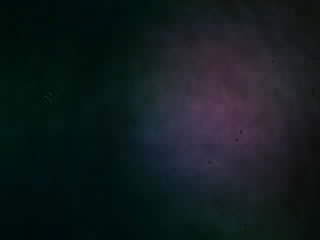
\includegraphics[width=0.5\linewidth]{pics/awb.jpg}
        \caption{Image with AWB}
    \end{subfigure}%
    \begin{subfigure}{0.5\textwidth}
    \centering
        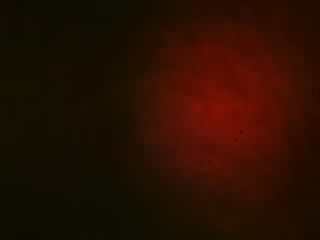
\includegraphics[width=0.5\linewidth]{pics/withoutawb.jpg}
        \caption{Image without AWB}
    \end{subfigure}
    \caption{Images of a laser beam caught with and without pinhole}
    \label{fig:AWB}
    \end{figure}
\end{itemize}
\subsection{Improved experiment}
As mentioned in the previous experiment, the stage was calibrated such that the sensor remains at the center of rotation of the rotational stage. The reference signal was chosen such that the same point of the beam is always measured. In order to make sure that the same point of the beam is measured with and without pinhole, the coordinate of the central diffraction pattern is stored for different angular positions for -45 to +45 and the reference signal is taken from this point. In order to detect the central region in the output, a function called \texttt{imfindcircles} is used\cite{imfindcircles}. This function finds circles in an image using using circular Hough transform. The readings for a specific angle are averaged and a logarithmic function is applied which is then passed to the \texttt{imfindcircles} function to detect the brightest possible circle with a radius of 3 pixels(This value was tuned such that the  central portion is detected with 100 percent accuracy). The detection process using this this method provided 100 percent accuracy for detection of the center of the central fringe pattern coordinate. This is illustrated in Figure \ref{fig:center_calib}. The Automatic gain controls and Automatic White balance features of the CMOS sensors were turned off by using suitable register settings mentioned in \cite{OV2640DS}. The Arduino was programmed to set the register values using I2C. The exposure was set at 500$\mu$s based on the exposure graph mentioned in the previous section.
\begin{figure}[!h]
\centering
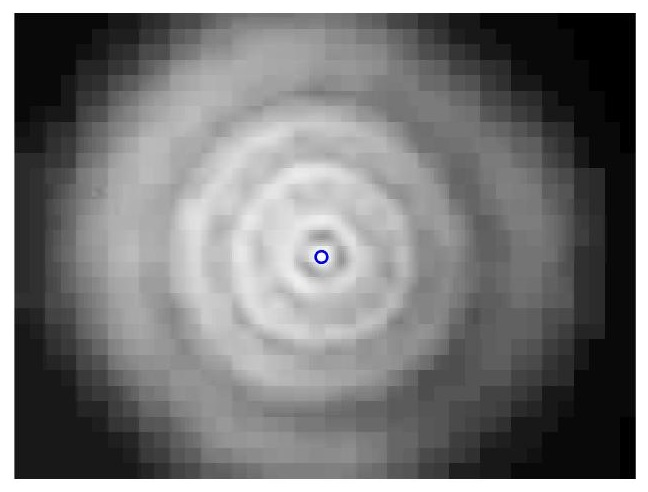
\includegraphics[scale=0.300]{pics/CentralRegionTracking.jpg}
\caption{Coordinate Detection for central region signal detection}
\label{fig:center_calib}
\end{figure}

In the first step of the experiment, the rotational stage is rotated from -45 to +45 degrees with pinhole, and the coordinates of the central diffraction pattern is stored in a variable. In the second step of the experiment, the pinhole is removed and the signal is taken for different angle from the coordinates mentioned in the previous step. After this, the signal is taken with different offset(from the central diffraction pattern) in the X-direction to make sure that all the pixels behave in the same manner. The graphs for 100 different pixel positions from the central position is shown in Figure \ref{fig:offset_calib}. From this graph,it can be seen that all the pixels in the same line exhibit the same behaviour with a slight shift in angular position peak. In figure \ref{fig:offset_calibY}, the response for different pixels in the Y-direction is shown. It can  be seen that there is a wider variation in the curve peak position. It can also be seen that all the pixels follow the same pattern with a slight shift in the peaks.
\begin{figure}[!h]
\centering
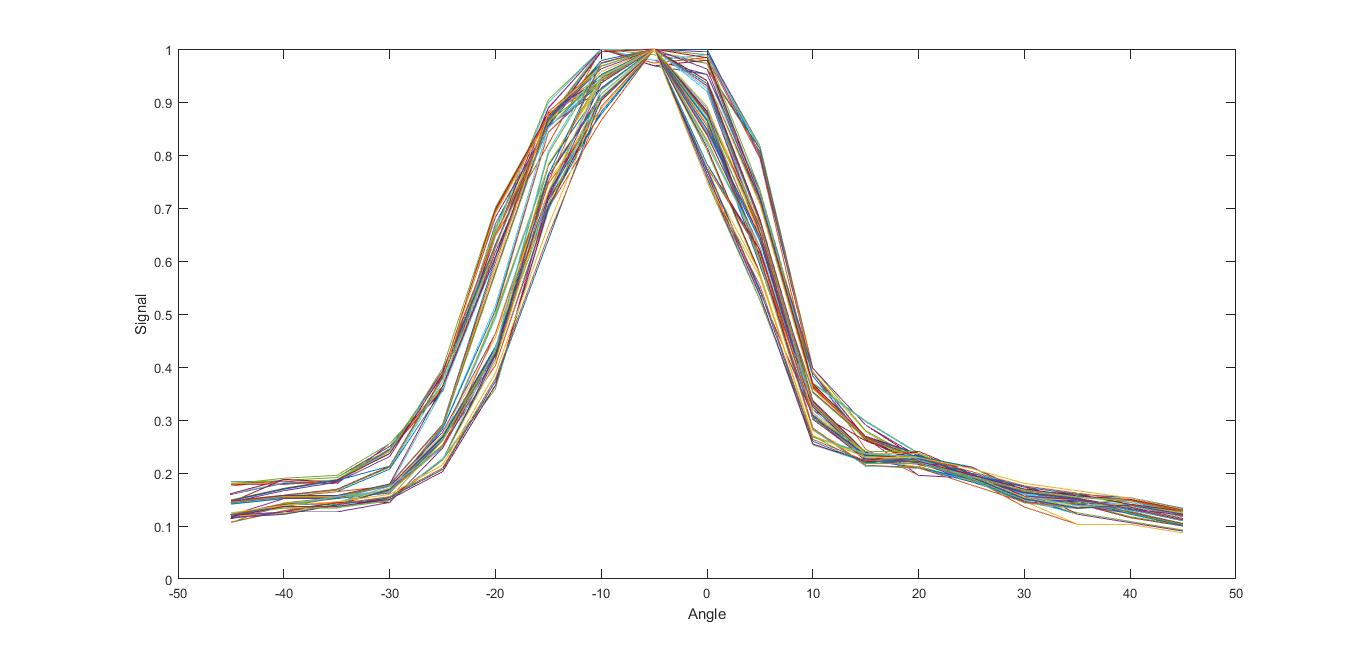
\includegraphics[scale=0.2125]{pics/ResponseOffset.jpg}
\caption{Response for 100 different offset pixel positions from central diffraction pattern in X-direction}
\label{fig:offset_calib}
\end{figure}

\begin{figure}[!h]
\centering
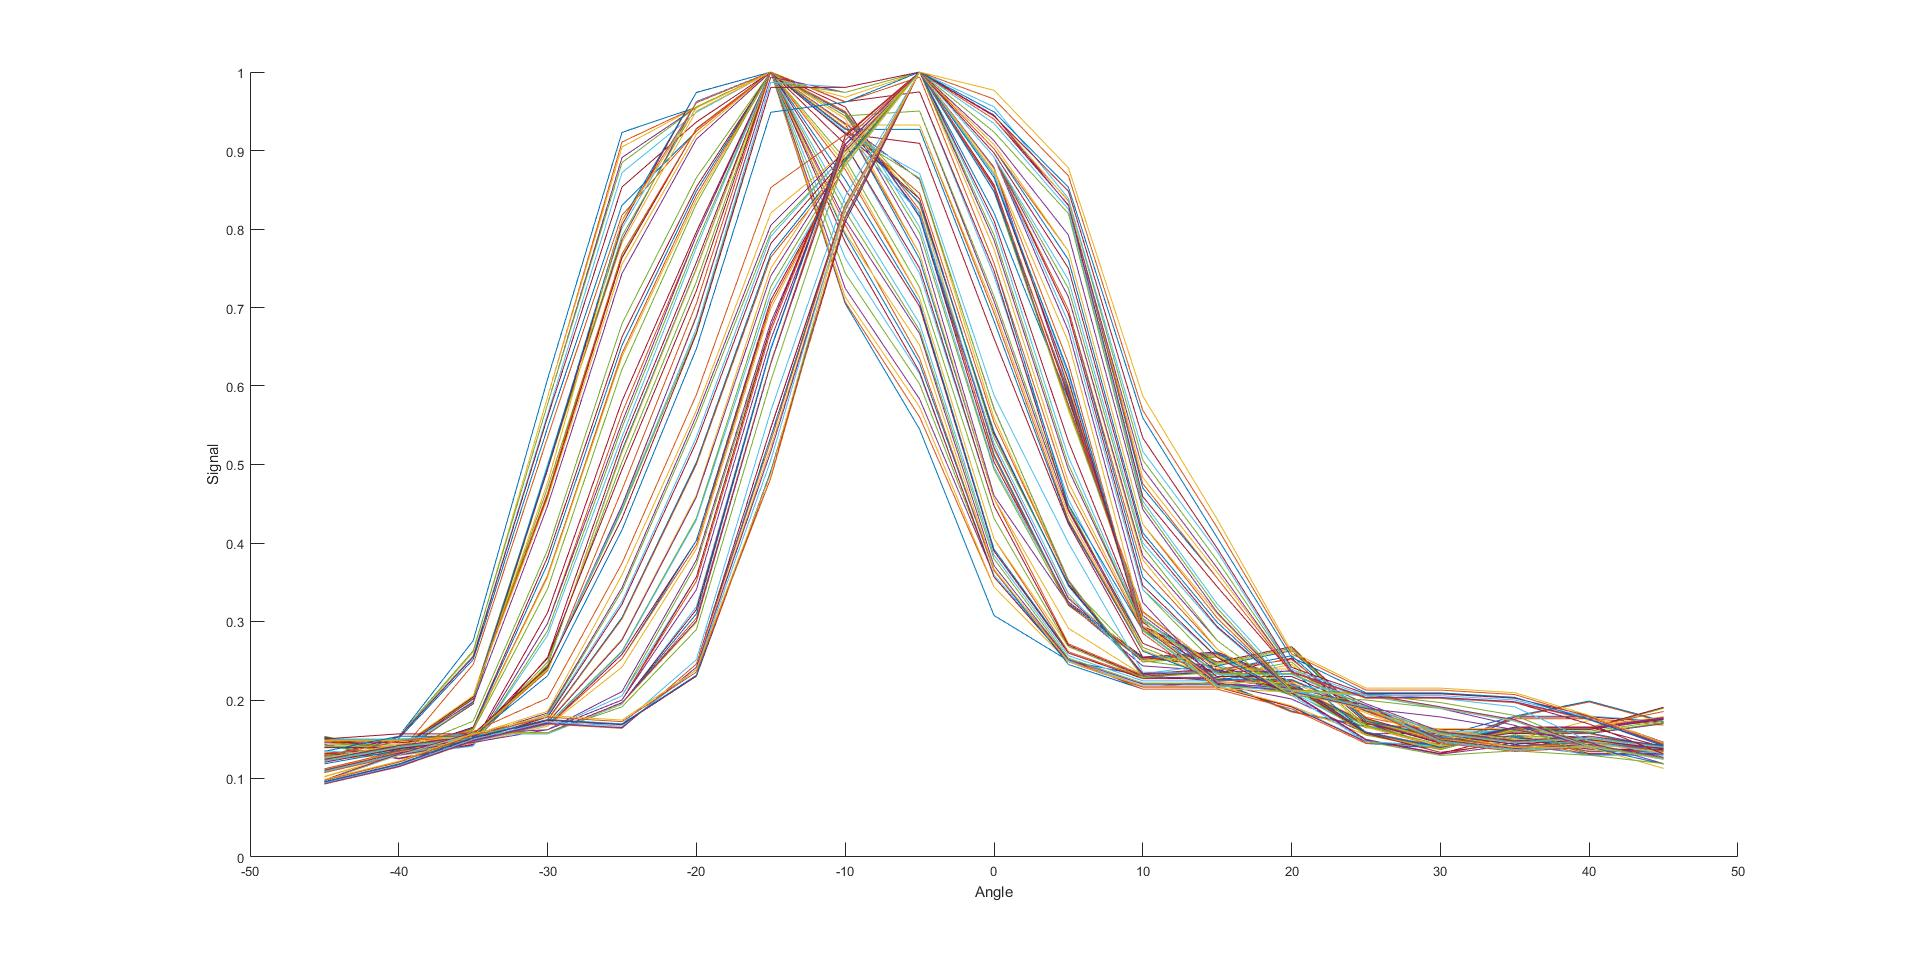
\includegraphics[scale=0.150]{pics/ResponseYOffset.jpg}
\caption{Response for 100 different offset pixel positions from central diffraction pattern in Y-direction}
\label{fig:offset_calibY}
\end{figure}

The peak positions for different pixel offset positions in the X and Y direction is shown in \ref{fig:peak_pixel_pos}. It can be seen that pixels in the same neighborhood have the same peak angular positions. The shift in peak is seen as we move across the detector. This can be attributed to the non-uniformity in the laser beam that is used for measuring the response of the pixels.
\begin{figure}[!h]
\centering
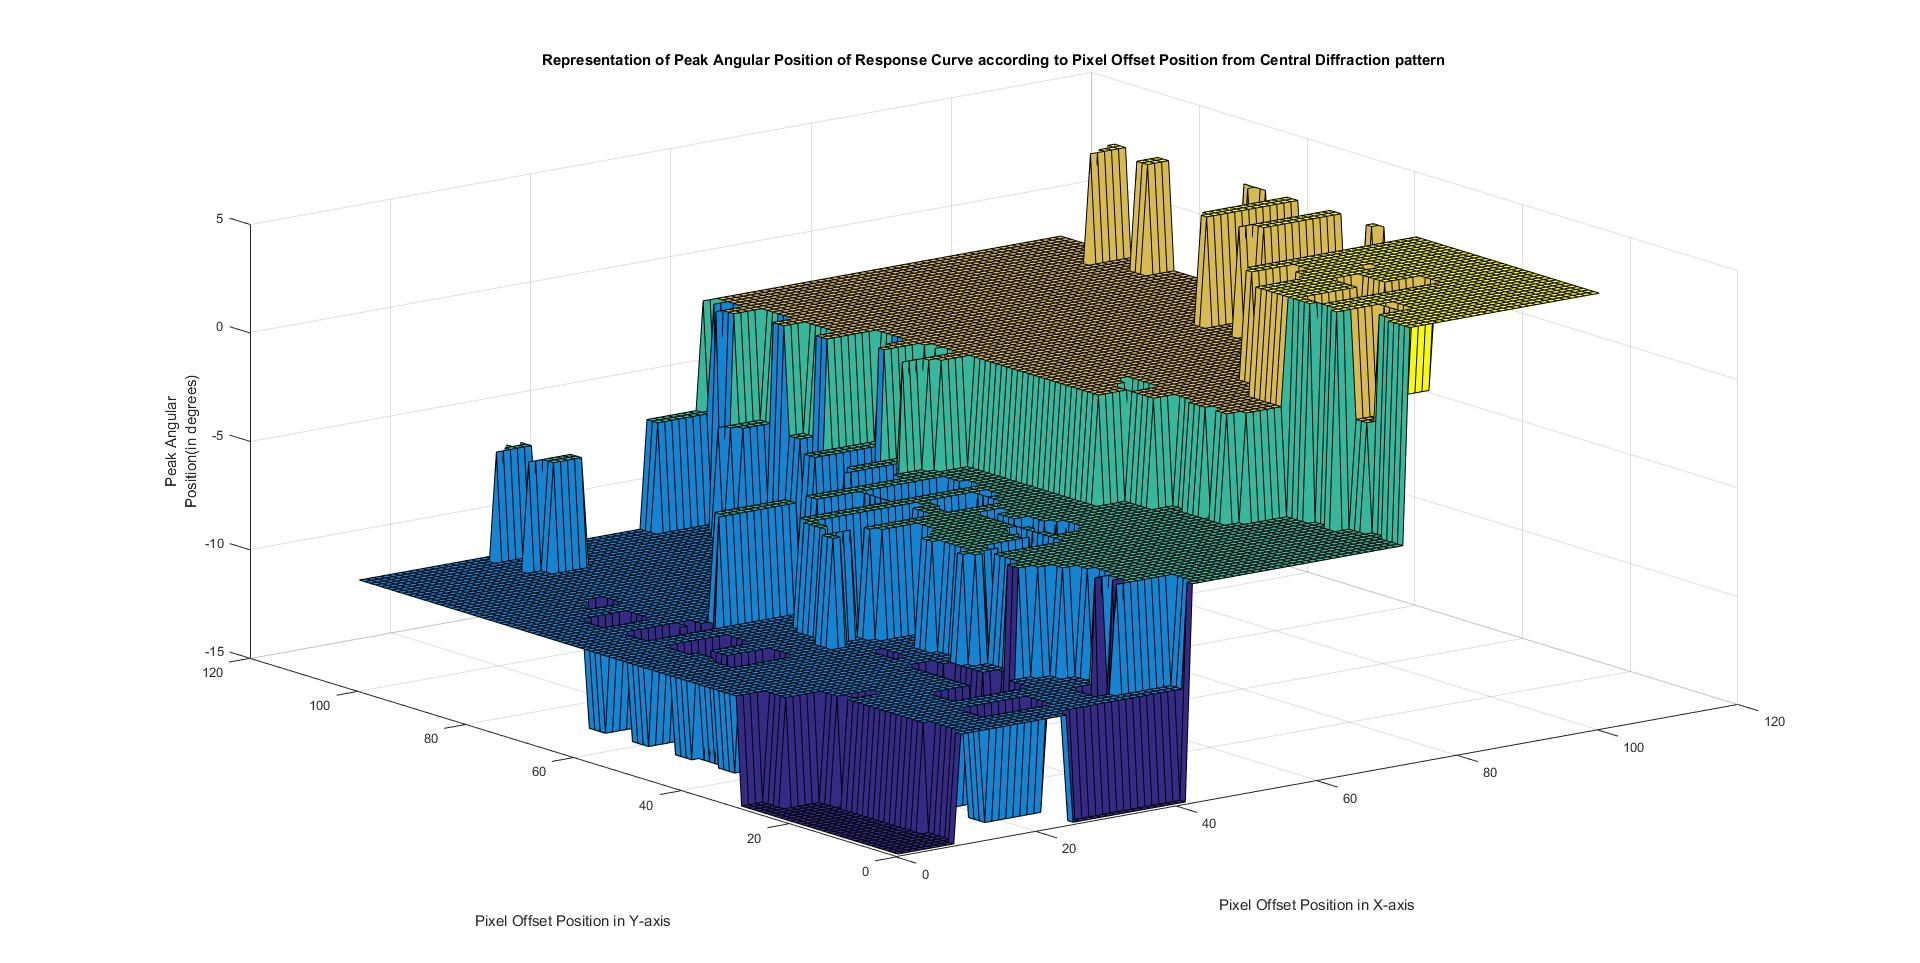
\includegraphics[scale=0.225]{pics/MeshPlotAngularPeak.jpg}
\caption{Peak Angular Positions for different Pixels}
\label{fig:peak_pixel_pos}
\end{figure}

The experiment is repeated for 10 times and the response is plotted only for the red channel as we have only red frequency light hitting the sensor beam. The final result after solving the problems mentioned in the previous section is shown in Figure \ref{fig:acceptance_final}.
\begin{figure}[!h]
\centering
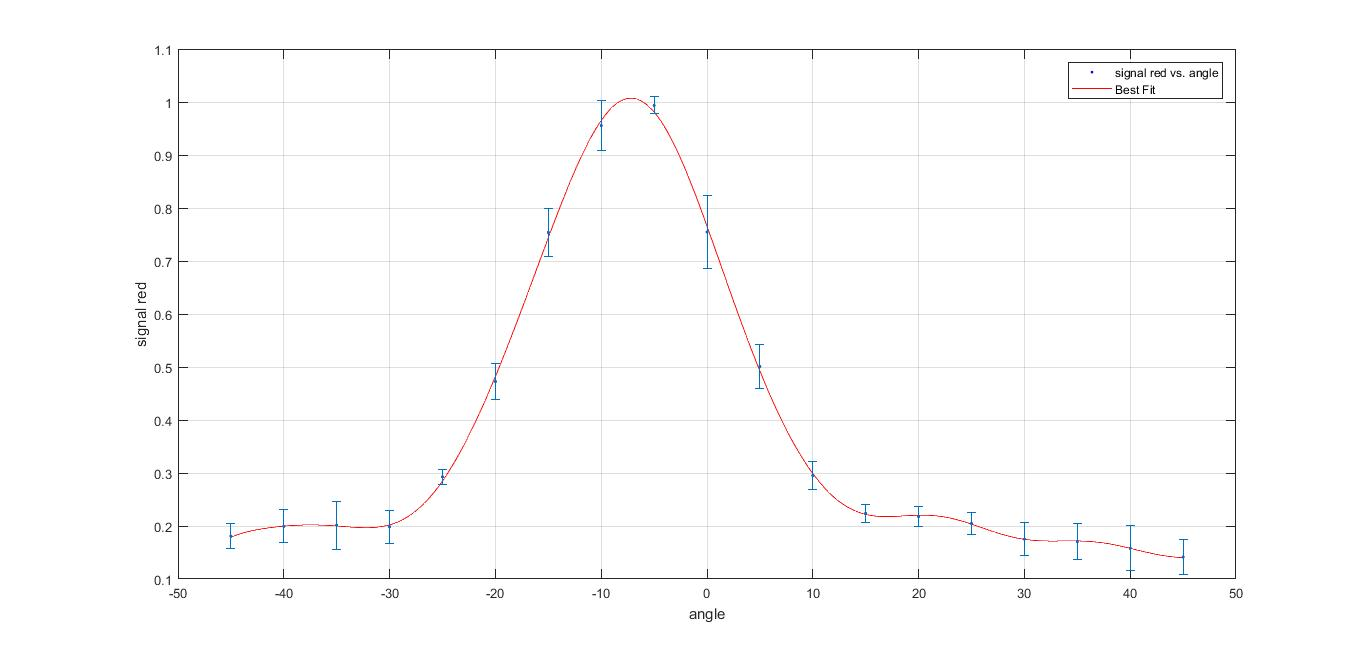
\includegraphics[scale=0.2125]{pics/FinalCRAExp.jpg}
\caption{Red Channel Response for Different Data Sets}
\label{fig:acceptance_final}
\end{figure}
There is less overlap in the subsequent angles and no points for excluded in the curve fitting process. The maximum standard deviation has reduced from 16 percent for angular position -20 to 6 percent for angular position 0. The peak of the curve is shifted towards -5 degrees because the maximum position of the laser beam occurs at -5 degree position of the rotational beam. This data needs to be incorporated into the simulation to see the effect of the acceptance cone of the sensor on the image reconstruction. This will be discussed in the subsequent section.
\section{Adding to Simulation}
The curve data that was obtained in the previous experiment was incorporated into the previously obtained simulation results. In order to incorporate the data, we need to generate a 2-dimensional matrix that would simulate the behavior of the acceptance cone effect on the re-construction. Since the behaviour will be in both the x and y directions, the 1-d curve was converted into 2-d by multiplying itself with it's transpose. This would generate a circular symmetric matrix that would generate the effect of the acceptance cone in both the x and y directions. This is shown in Figure \ref{fig:curve_sim}.
\begin{figure}[!h]
\centering
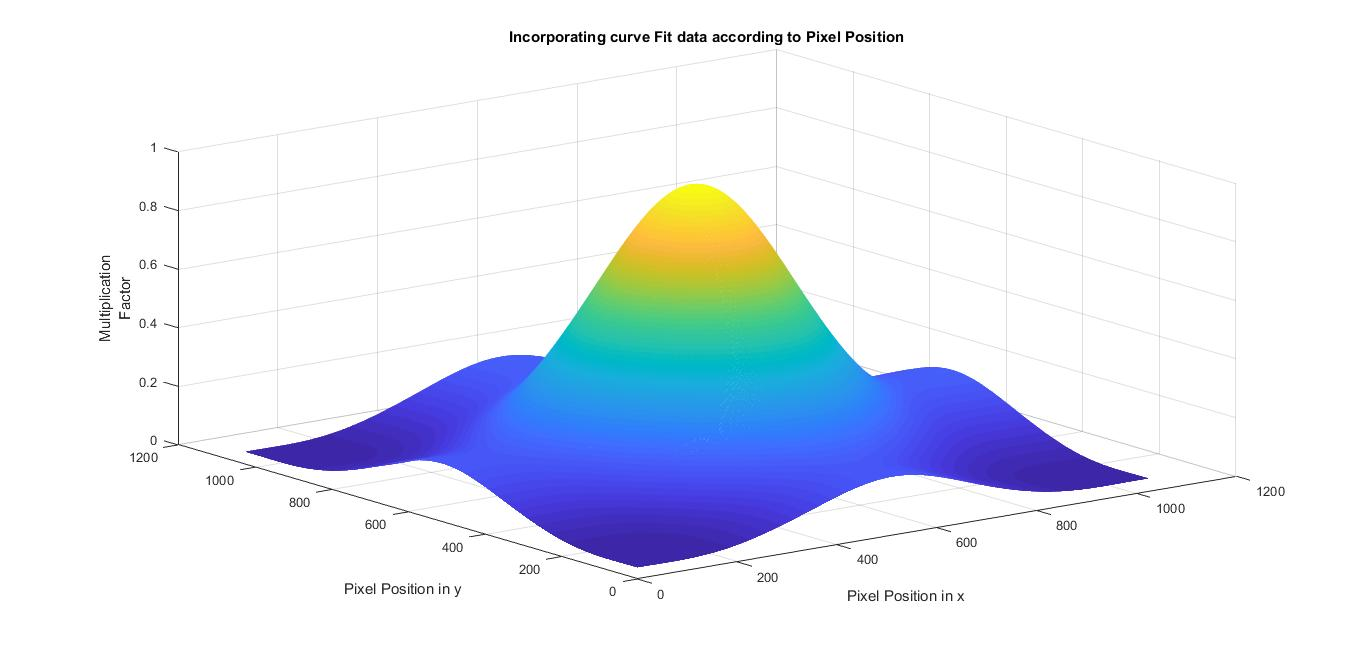
\includegraphics[scale=0.25]{pics/AcceptanceConeCurveFit.jpg}
\caption{Fitted Curve Data into simulation}
\label{fig:curve_sim}
\end{figure}
This matrix was multiplied with the original image to simulate the effect of angle acceptance on the image reconstruction. This was tried with the simulation results that simulate the effects of diffraction to simulate as close to a real world. The source image is shown in Figure \ref{fig:Orig}. The reconstruction effects simulated after reconstruction is shown in Figure \ref{fig:Rec_Diff}. It can be seen that most of the source image is reconstructed with slight loss in information only with diffraction. Once we incorporate the effects of acceptance cone into the simulation, it can be seen that only a portion of the original image can be reconstructed which is indicated by the rectangular box in Figure \ref{fig:Rec_Acc}. 
This would be the actual field of view in the real world. The actual area of the sensor which can be used is drastically reduced by approximately 50 percent. In order to find the angular field of view, the positions of the rectangular box must be correlated with the fitted matrix curve discussed. On doing this, it can be found that the area in the rectangular box corresponds to an angle from -21.7 to +21.7.

\begin{figure}[]
\centering
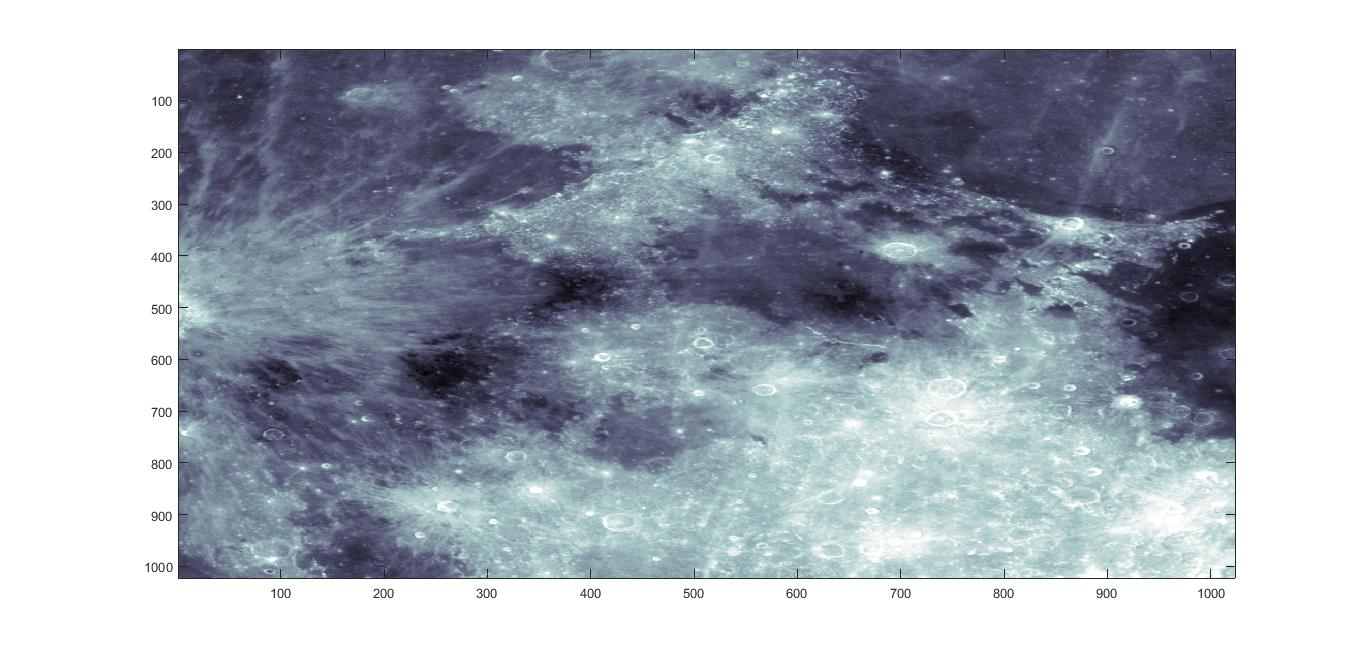
\includegraphics[scale=0.25]{pics/OriginalImage.jpg}
\caption{Source Image Cut from Moon}
\label{fig:Orig}
\end{figure}

\begin{figure}[]
\centering
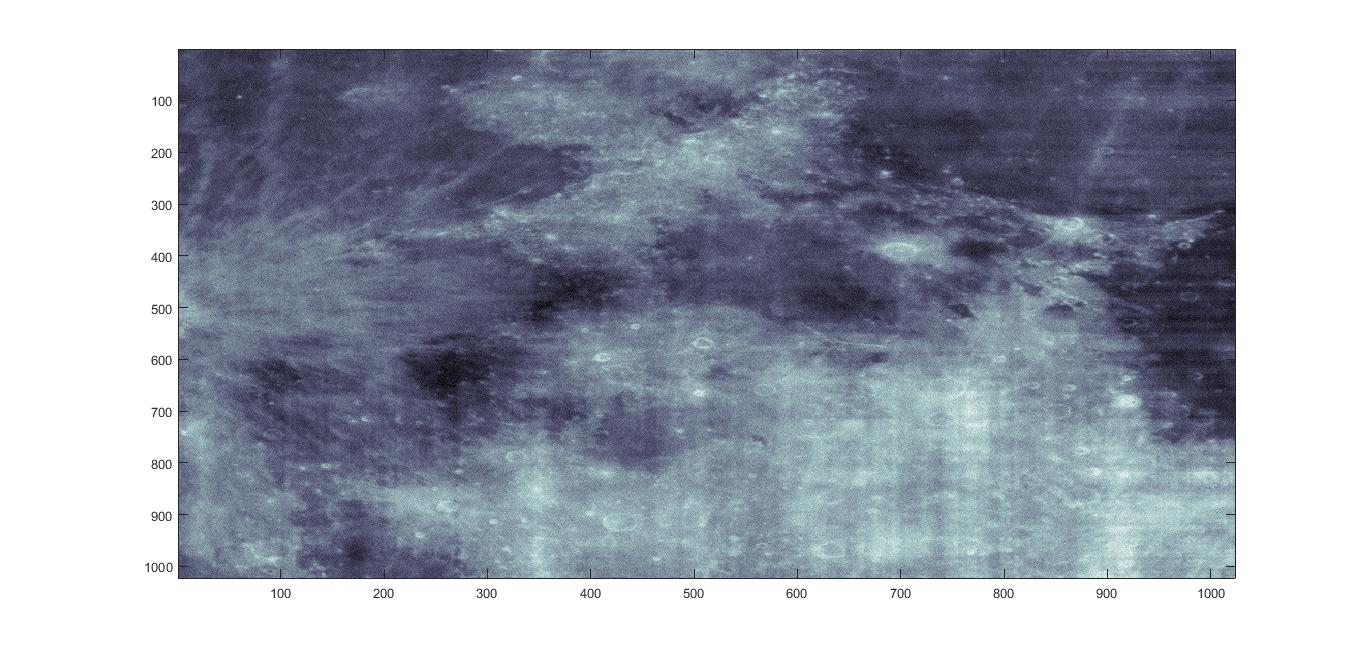
\includegraphics[scale=0.25]{pics/OriginalImageDiffRec.jpg}
\caption{Reconstruction with Diffracted Mask}
\label{fig:Rec_Diff}
\end{figure}

\begin{figure}[]
\centering
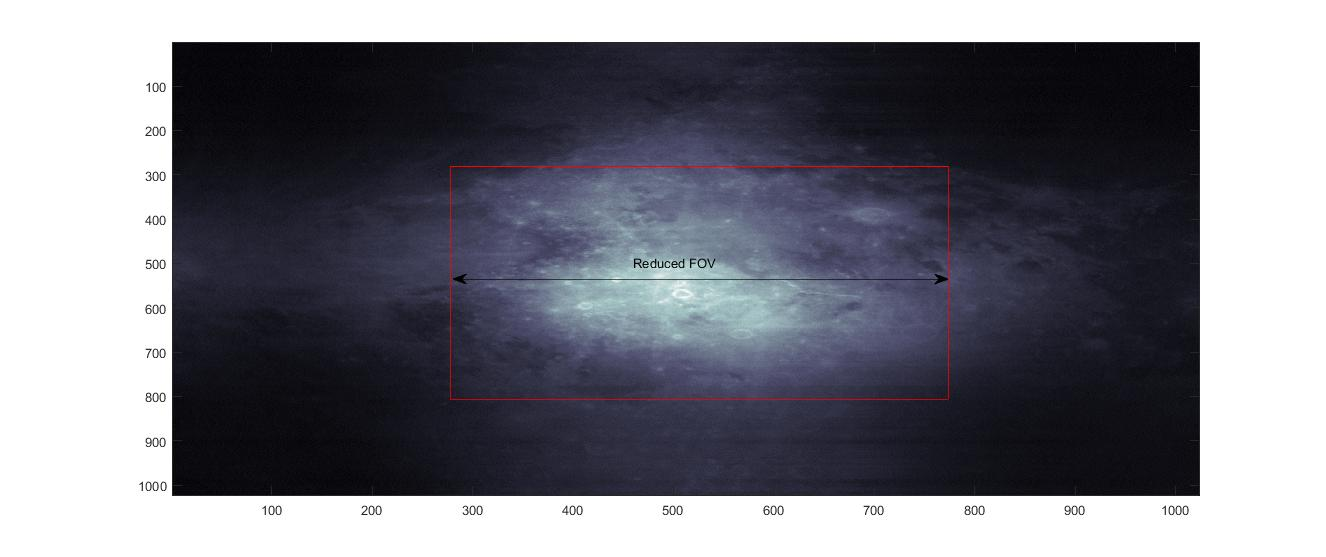
\includegraphics[scale=0.25]{pics/ImageRecWithAcc.jpg}
\caption{Reconstruction with Diffracted Mask and Curve Data}
\label{fig:Rec_Acc}
\end{figure}

\section{Spatial Light Modulators}
A spatial light modulator (SLM) is an object that imposes some form of spatially varying modulation on a beam of light\cite{SLMWiki}.SLMs can be controlled by computer controlled software and it would be possible to generate patterns on the SLM that could modulate phase or the intensity of the beam or both simultaneously. An advantage of using an SLM over designing a lithographic mask is that it would be possible to test out different designs of masks quickly in order to find out an optimal mask configuration that would be suitable to our setup. In our design of the lensless imager, it must be possible to block and allow light in a certain binary pattern. A transmissive SLM would suit the purpose of simulating different mask patterns. For this purpose, a holoeye LC2012 SLM was used 

\begin{figure}[ht]
\centering
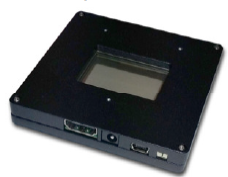
\includegraphics[width=0.5\textwidth]{pics/slm}
\caption{HoloEye LC2012 SLM}
\label{fig:slm}
\end{figure}
